\documentclass[12pt]{extarticle}
\usepackage{tempora}
\usepackage[T1, T2A]{fontenc}
\usepackage[utf8]{inputenc}
\usepackage[english, ukrainian]{babel}
\usepackage{geometry}
\usepackage{graphicx}
\usepackage{multirow}
\usepackage{multicol}
\usepackage{float}
\graphicspath{{/home/artem/Pictures}}
\geometry
{
    a4paper,
    left=30mm,
    top=15mm,
    right=20mm,
    bottom=15mm,
}

\begin{document}
\begin{titlepage}
    \begin{center}
        \textbf{\normalsize{\MakeUppercase{
            Міністерство Освіти і науки України
            Національний університет "Львівська політехніка"
        }}}

        \begin{flushright}
        \textbf{ІКНІ}\\
        Кафедра \textbf{ПЗ}
        \end{flushright}
        \vspace{15mm}

        \includegraphics[width=0.4\textwidth]{lpnu_logo.png}

        \vspace*{\fill}

        \textbf{\normalsize{\MakeUppercase{Звіт}}}
            
        До лабораторної роботи №7

        \textbf{на тему:} “Складення та відлагодження циклічної програми мовою асемблера
мікроконтролера Cortex-M4”

        \textbf{з дисципліни:} “Архітектура комп’ютера”
            
        \vspace*{\fill}

        \begin{flushright}

            \textbf{Лектор:}\\
            доцент кафедри ПЗ\\
            Крук О.Г.\\
            \vspace{12pt}

            \textbf{Виконав:}\\
            студент групи ПЗ-24\\
            Губик А. С.\\
            \vspace{12pt}

            \textbf{Прийняв:}\\
            доцент кафедри ПЗ\\
            Задорожний І. М.\\
        \vspace{12pt}
        \end{flushright}

        Львів -- 2023
            
            
    \end{center}
\end{titlepage}

\textbf{Тема роботи:}Складення та відлагодження циклічної програми мовою асемблера
мікроконтролера Cortex-M4

\vspace{12pt}

\textbf{Мета роботи:} ознайомитись на приладі циклічної програми з основними
командами асемблера процесорів Cortex- M3/M4; розвинути
навики складання програми з вкладеними циклами;
відтранслювати і виконати покроково в режимі
відлагодження програму, складену відповідно до свого
варіанту; перевірити виконання тесту.

\subsection*{Індивідуальне завдання}

1. Обчисліть скалярний добуток 1-го і 5-го рядків.

2.Обчисліть кількість і суму елементів 9-го стовпця, які
задовільняють вказаній умові

3.$b < a_i < c$

\subsection*{Теоретичні відомості}
Для того, щоб створити новий проект в середовищі розроблення програм Keil
μVision в меню Project треба вибрати команду «New μVision Project». Відкриється вікно
створення проекту «Create New Project», в якому необхідно, використовуючи дерево
каталогів, вказати потрібну папку. Якщо папка для проекту ще не створена, середовище
μVision дозволяє зробити це. Не виходячи з вікна створення проекту, потрібно
звичайними засобами операційної системи перейти у відповідну папку і створити в ній
нову папку. Про всяк випадок ім’я доцільніше вводити латинськими буквами. Ім’я
проекту може співпадати з іменем папки.
Тут же появиться вікно «Select Device for Target 'Target 1' »(«Виберіть цільовий
пристрій, 'Мета 1' »), в якому необхідно вказати для якого ядра мікропроцесора буде
призначена програма. Розкрийте список ARM і виберіть ARMCM4FP – процесор ARM
Cortex M4 з арифметичним співпроцесором.
Після вибору процесорного ядра відкриється вікно менеджера оточення реального
часу виконання Manage Run-Time Environment. Перша позиція містить компоненти
програмного інтерфейсу мікроконтролерів Cortex, які помітно прискорюють і
полегшують програмування мовою високого рівня С/С++. Серед них: заголовочні
файли з визначеннями регістрів периферійних пристроїв; засоби абстрактного доступу
до них; приклади. Друга позиція дозволяє під'єднати уніфіковані драйвери інтерфейсів,
такі як драйвер Ethernet, флеш-пам'яті тощо. Інші позиції також надають додаткові опції
програмістам мовою С/С++, починаючи від стартових файлів і закінчуючи підтримкою
графіки, USB-інтерфейсів та інше.
Для програмування мовою асемблера, тим більше на перших порах, можна
опустити всі додаткові можливості, натиснувши відразу (внизу вікна) клавішу «OK».
Новий проект буде створено і відображено у вікні проектів з ім'ям «LR11» (рис. 1). Для
даного проекту зазначено один цільовий пристрій Target 1 на базі вибраного процесора
Cortex-M4F. У вікні проектів показана перша група початкових файлів проекту - «Source
Group 1». Зазвичай в проекті достатньо однієї групи початкових файлів, однак в окремих
випадках їх може бути кілька. Крім того, для кожної з груп початкових файлів можна
встановлювати свої опції (налаштування) середовища.
\subsection*{Хід роботи}

\paragraph{1.}Програма що виводить П.І.Б.

\begin{verbatim}
    ; ????????? ?????? ?????? MyCode
	AREA MyCode, CODE, ReadOnly
; ????????? ????? ????? ? ???????? ???????
	ENTRY
; ????????? ????? ????? ?????????? ???????
	EXPORT MyProg
MyProg
PREPARE_TO_TRANSPOSE
	LDR r2, = 6  ; ?????
	LDR r3, = 9 ; ???????
	LDR r7, = 4  ; DCD size
	LDR r4, = 0  ; ????????? ??????? ??????

TRANSPOSE
	LDR r5, = 0  ; ????????? ??????? ????????? ?????
TRANSPOSE_ROW
	LDR r0, = array 
	LDR r1, = transponed
	MUL r6, r5, r3 		; ?????????? ??????????? ?????
	ADD r6, r4 			; ?????????? ??????????? ????????
	MUL r6, r6, r7 		; ??????? ?? ?????? ????????
	ADD r0, r6			; ?????????? ?? ???????????? ????????
	MUL r6, r4, r2		; ?????????? ??? ? ????????, ? ??? ????????????
	ADD r6, r5
	MUL r6, r6, r7
	ADD r1, r6
	LDR r6, [r0]		; ???????????? ??????? ? ???????
	STR r6, [r1]		; ?????????? ???? ? ?????? ???????
	ADD r5, #1			; ????????????? ????????? ??????? ????????? ?????
	CMP r5, r2
	BNE TRANSPOSE_ROW	; ? ???? ?????????? ???? ????????? ????? ????????? ?????????? ??? ? ?????????? ??????
	ADD r4 , #1
	CMP r4 , r3
	BNE TRANSPOSE
	
	LDR r0, = array
	LDR r1, = array		; ???????????? ??????
	ADD r0, #4*9*0		; ?????????? ?? 3 ?????
	ADD r1, #4*9*4		; ?????????? ?? 4 ?????
	LDR r2, = 9		; ????????? ??????
	LDR r3, = 0
; ?????????? ????????? ???????
DOT
	LDR r4, [r0], #4
	LDR r5, [r1], #4
	MUL r6, r4, r5
	ADD r3, r6
	SUB r2, #1
	CMP r2, #0
	BNE DOT
	
	LDR r7, = dotProduct
	STR r3, [r7]


	LDR r0, = array
	ADD r0, #4*8		; ?????????? ?? 9 ???????? 1 ?????
	LDR r1, = 4			; ????????? ??????
	LDR r3, = 0
	LDR r4, = 0
COND
	LDR r2, [r0], #4*9	; ???. ??????? ? ??????? ?? ??????? ?? ????. ?????
	CMP r2, #-67
		BLE NEXT
	CMP r2, #94
		BGE NEXT
	ADD r3, #1		; ? ???? ????????????? ???? ?????????? ????????? ?? ????
	ADD r4, r2
NEXT	
	SUB r1, #1
	CMP r1, #0
	BNE COND

	LDR r5, = amount
	LDR r6, = sum
	STR r3, [r5]
	STR r4, [r6]

Stop 		B Stop

	ALIGN
; ????????? ?????? ????? ? ???'???
	AREA MyData, Data, ReadOnly
	EXPORT array
array 		DCD -17,  32, -51,  24, -11,  14,  71, -62, 85
			DCD  30, -20, -47,  63,  12,  52,  36,  12, 11
			DCD  44, -23, -85,  12,  93,  24, -46,  38, 13
			DCD -23, -18,  16,  19,  24,  56, -71, -12, 15
			DCD  44, -23, -85,  12,  93,  24, -46,  38, 13
			DCD -23, -18,  16,  19,  24,  56, -71, -12, 15


; ????????? ?????? ????? ? ??????????? ???'???
	AREA MyData1, Data, ReadWrite
	EXPORT transponed
	EXPORT dotProduct
	EXPORT sum
	EXPORT amount

; ????????????? ? ??? ????? ??? ??????????
; ????????? ????????? ? ?????????? ????
transponed 		SPACE 6 * 9
dotProduct		SPACE 4
sum			SPACE 4
amount		SPACE 4

; ?????? ????????????? ??????
	END

\end{verbatim}

\vspace{12pt}
\begin{figure}[H]
    \centering
    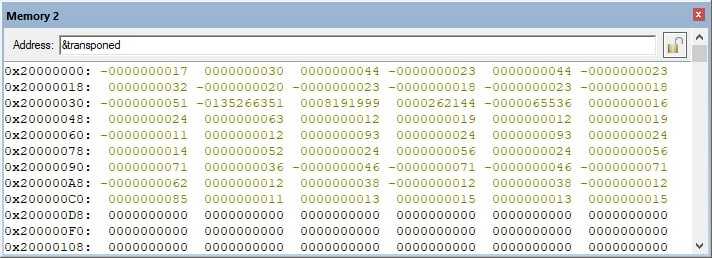
\includegraphics[width=0.90\textwidth]{array.jpg}
    \caption{}
\end{figure}

\vspace{12pt}
\begin{figure}[H]
    \centering
    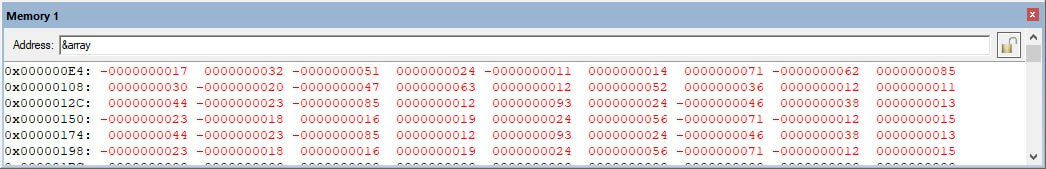
\includegraphics[width=0.90\textwidth]{transponed.jpg}
    \caption{}
\end{figure}

\vspace{12pt}
\begin{figure}[H]
    \centering
    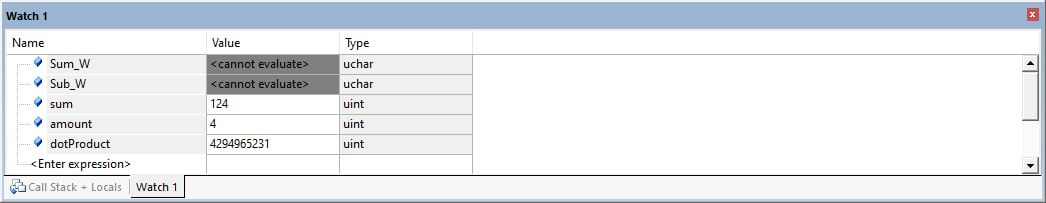
\includegraphics[width=0.90\textwidth]{vars.jpg}
    \caption{}
\end{figure}

\vspace{12pt}

\subsection*{Висновок} 
Я освоїв базові можливості асеблера на архітектурі ARM.

\end{document}